% Created 2023-02-08 Wed 12:56
% Intended LaTeX compiler: xelatex
\documentclass[presentation]{beamer}
\usepackage{graphicx}
\usepackage{longtable}
\usepackage{wrapfig}
\usepackage{rotating}
\usepackage[normalem]{ulem}
\usepackage{amsmath}
\usepackage{amssymb}
\usepackage{capt-of}
\usepackage{hyperref}
\usepackage[scheme=plain]{ctex}
\usetheme{Madrid}
\author{Jinghui Hu}
\date{\textit{<2023-02-02 Thu 11:21>}}
\title{GroupBy语句实现原理探索}
\hypersetup{
 pdfauthor={Jinghui Hu},
 pdftitle={GroupBy语句实现原理探索},
 pdfkeywords={},
 pdfsubject={},
 pdfcreator={Emacs 28.2 (Org mode 9.5.5)},
 pdflang={English}}
\begin{document}

\maketitle
\begin{frame}{Outline}
\tableofcontents
\end{frame}



\section{示例数据介绍}
\label{sec:org12a3c9f}
\begin{enumerate}
\item 示例数据库 \href{https://dev.mysql.com/doc/employee/en/employees-installation.html}{Employees Sample Database} | \href{https://github.com/datacharmer/test\_db}{Github}
\begin{center}
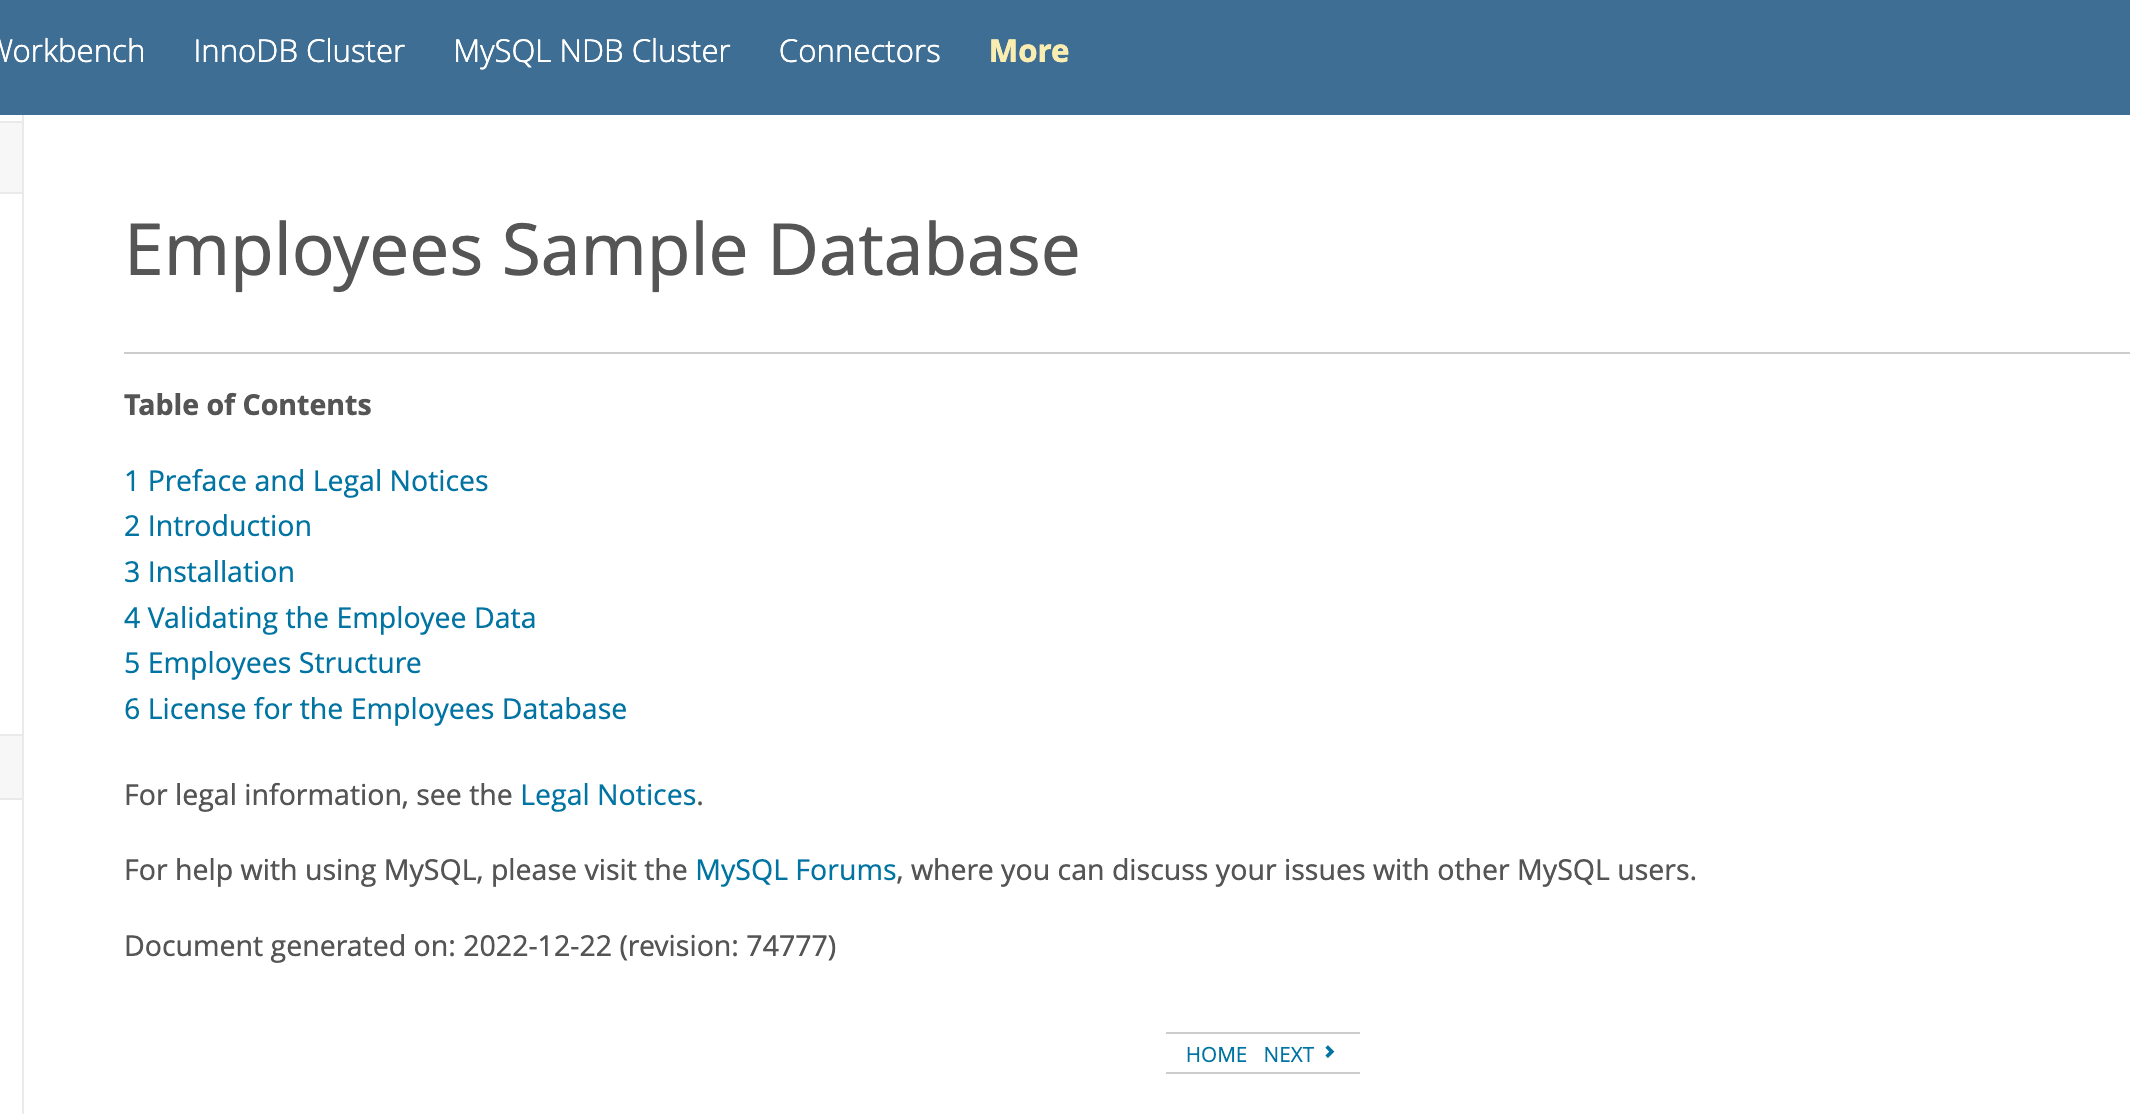
\includegraphics[width=.9\linewidth]{../static/image/2023/0208/125223.png}
\end{center}
\item 导入测试样例数据
\begin{verbatim}
mysql < employees.sql
\end{verbatim}
\item 数据库的 Schema
\end{enumerate}
\begin{center}
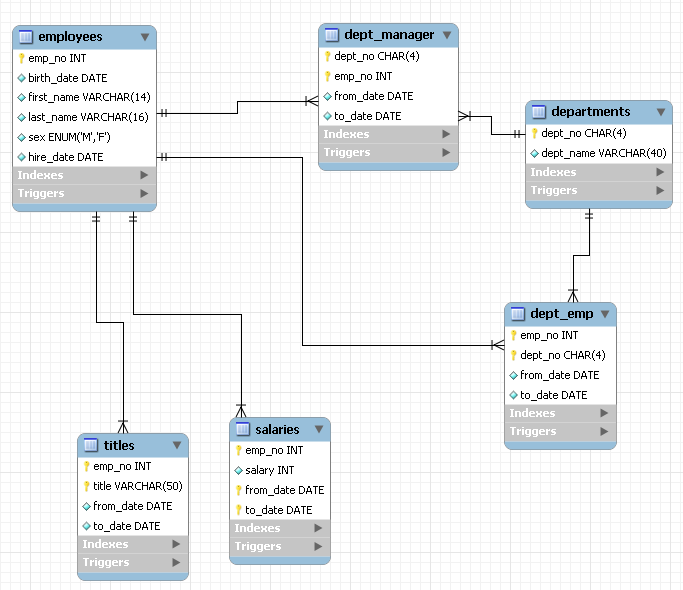
\includegraphics[width=.9\linewidth]{../static/image/2023/0208/103345.png}
\end{center}
\section{研究问题}
\label{sec:org803c226}
\begin{frame}[label={sec:org06b9ce9},fragile]{查看一下 employees 的表结构}
 \begin{verbatim}
show create table employees\G
\end{verbatim}

\begin{verbatim}
*************************** 1. row ***************************
       Table: employees
Create Table: CREATE TABLE `employees` (
  `emp_no` int NOT NULL,
  `birth_date` date NOT NULL,
  `first_name` varchar(14) NOT NULL,
  `last_name` varchar(16) NOT NULL,
  `gender` enum('M','F') NOT NULL,
  `hire_date` date NOT NULL,
  PRIMARY KEY (`emp_no`)
) ENGINE=InnoDB DEFAULT CHARSET=utf8mb4 COLLATE=utf8mb4_0900_ai_ci
\end{verbatim}
\end{frame}

\begin{frame}[label={sec:org77b559c},fragile]{选取 10 条示例数据}
 \begin{verbatim}
select * from employees limit 10;
\end{verbatim}

\begin{center}
\begin{tabular}{rrlllr}
emp\_no & birth\_date & first\_name & last\_name & gender & hire\_date\\
\hline
10001 & 1953-09-02 & Georgi & Facello & M & 1986-06-26\\
10002 & 1964-06-02 & Bezalel & Simmel & F & 1985-11-21\\
10003 & 1959-12-03 & Parto & Bamford & M & 1986-08-28\\
10004 & 1954-05-01 & Chirstian & Koblick & M & 1986-12-01\\
10005 & 1955-01-21 & Kyoichi & Maliniak & M & 1989-09-12\\
10006 & 1953-04-20 & Anneke & Preusig & F & 1989-06-02\\
10007 & 1957-05-23 & Tzvetan & Zielinski & F & 1989-02-10\\
10008 & 1958-02-19 & Saniya & Kalloufi & M & 1994-09-15\\
10009 & 1952-04-19 & Sumant & Peac & F & 1985-02-18\\
10010 & 1963-06-01 & Duangkaew & Piveteau & F & 1989-08-24\\
\end{tabular}
\end{center}
\end{frame}

\begin{frame}[label={sec:org629dfda},fragile]{问题引出}
 研究👇🏻 语句中 group by 的执行流程
\begin{verbatim}
select
  last_name,
  count(*) total
from
  employees
group by
  last_name
order by
  2 desc
limit 10;
\end{verbatim}
\end{frame}

\section{整体执行流程}
\label{sec:org8ed9be6}
\begin{verbatim}
use strict;
use warnings;

my $cid = 8;
my $fout = "/tmp/mysqld-thd-$cid.txt";
open(FIN, '<:encoding(UTF-8)', "/tmp/mysqld.trace") or die;
open(FOUT, '>', $fout) or die;

while (my $line = <FIN>) {
    if ($line =~ /^T\@$cid/) {
        print FOUT $line;
    }
}

close(FOUT);
$fout;
\end{verbatim}
\end{document}